Es blieb zu wenig Zeit, um die tausenden verfügbaren Endstufen einzeln zu evaluieren. Deshalb wurde hier mit ChatGPT eine AI eingesetzt, welche mit folgendem Prompt getriggert wurde:\\
\begin{center}
	\begin{parbox}[][][]{\textwidth*3/4}
		{\textit{\dotfill\\recommend me some D-Class loudspeaker driver chips which can handle at least 7.5 Watts and accepts digital inputs such as I2S or TDM and has an integrated limiter}\\.\dotfill.}
	\end{parbox}
\end{center}\vspace{3mm}
Die Antwort der KI war:\\.\dotfill.\\\textit{\textbf{{\Large Recommendations (short list})}\\
	1) \textbf{TAS2770 (TI)} — Mono, 20 W class-D, digital in, speaker-protection / peak limiter
	\\Power: up to 20 W (mono) (depends on VDD and load).\\Digital input: I2S/TDM compatible (host supplies I2S / TDM).\\Limiter/protection: built-in speaker voltage \& current sensing and a battery-tracking peak-voltage limiter / SmartAmp style protections.\\Supply: 4.5–18 V (check datasheet graphs for exact conditions).\\Good for: battery-powered speakers, portable devices where speaker protection \& headroom tracking matter.\\2) \textbf{TAS5720 / TAS5720x (TI)} — Mono, ~20 W class-D, digital/TDM input, protection features\\Power: ~20 W (mono) (VDD and load dependent).\\Digital input: supports I2S / TDM (up to multi-device arrays).\\Limiter/protection: includes speaker protection and status/diagnostics; datasheet describes the SAIF serial audio interface and protection features.\\Supply: 4.5–26.4 V (device variant dependent).\\Good for: simple mono modules and multichannel TDM systems.\\3) \textbf{TAS5760 / TAS5760L(TI)} — Stereo, closed-loop digital-in Class-D, integrated digital clipper/limiter\\Power: stereo ≈21 W / ch (mono bridged higher) depending on supply/impedance.\\Digital input: native I2S input (digital-in family).\\Limiter/protection: integrated digital clipper / closed-loop speaker sensing and diagnostic features.\\Supply: ~4.5–16 V (variant dependent).\\Good for: stereo compact systems that need closed-loop control and built-in clipping/limiting. 
	Texas Instruments\\4) \textbf{TAS2781 (TI)} — Mono digital-in SmartAmp, ~25 W, integrated speaker-protection \& real-time algorithms\\Power: ~25 W (mono) (depends on supply and load).\\Digital input: I2S from host; integrated DSP for processing and protection.\\Limiter/protection: TI “SmartAmp” speaker protection algorithms and I/V sense for real-time protection.\\Supply: 4.5–23 V.\\Good for: louder mono drivers where sophisticated protection and DSP control are wanted.\\5) \textbf{TAS2557 / TAS255x family (TI)} — Integrated DAC + Class-D with SmartAmp protection (lower power members available ~5–10 W up to bigger SoCs)\\Power: some family members are in the >7.5 W range (check exact part variant).\\Digital input: on-chip DAC + I2S input.\\Limiter/protection: TI SmartAmp/clipper features, speaker sensing on higher-end members.\\Good for: integrated DAC + amp single-chip solutions for compact designs.\\6) \textbf{SSM3515 (Analog Devices)} — Mono digital-input Class-D, up to ~25–31 W (depending on VDD \& load), with AGC/limiting features\\Power: datasheet shows ~25–31 W under certain VDD / load / THD conditions (check graphs).\\Digital input: supports digital audio interface; I2C control for gain/setting.\\Limiter/protection: supply-monitoring AGC function and other protection features (useful as a limiter/level control).\\Good for: applications needing a digital-in amp with AGC/limiting.}\\.\dotfill.\\
\subsubsection{Kurzevaluation}Obwohl die KI anscheinend bevorzugt die grösseren Hersteller (Texas Instruments und Analog Devices) auflistet und hier eher TI-Produkte auswählt, wurde die Antwort als wertvoller Input angesehen. Nach einer kurzen Recherche wurde klar, dass einige bereits ältere Modelle vorgeschlagen wurden. Jedoch haben sich bei genauerer Evaluation zwei Modelle als potentiell Interessant für dieses Projekt erwiesen: Der TAS2781 und TAS5720. Abbildungen \ref{pic:blockschaltbild_TAS2781} und \ref{pic:blockschaltbild_TAS5720} zeigen jeweils das Blockschaltbild und Tabelle \ref{tab:Vergleich_TAS2781_TAS5720} zeigt eine Gegenüberstellung der Kennzahlen.\\
Die anderen Modelle fielen aus folgenden Gründen weg:
\begin{itemize}
	\item \textbf{TAS2770}: EOL, der Nachfolger \textbf{TAS2780} ist ähnlich wie der \textbf{TAS2781}, besitzt jedoch keinen internen DSP für den Lautsprecherschutz.
	\item \textbf{TAS2557}: EOL, die Nachfolger sind eher zu wenig Leistungsfähig (\textit{ca. }6.5W).
	\item \textbf{TAS5760}: Reiner Stereo-Amp, es können daher nicht 6 Kanäle gleichzeitig verstärkt werden.
	\item \textbf{SSM3515}: Besitzt zwar die Möglichkeit bis zu 16 TDM-Kanäle auszulesen, es können aber nur maximal 4 verschiedene I2C-Adressen konfiguriert werden, wodurch die TDM-Slot Zuweisung nicht möglich ist.
\end{itemize}
Aus Erfahrungswerten war auch die Firma \href{https://www.cirrus.com/}{Cirrus Logic} als Hersteller für Audio-ICs bekannt. Jedoch sind deren Endstufen CS35L42 und CS35L45 mit 5.3 und 6.8 Watt ein wenig zu Leistungsschwach.
\begin{figure}[H]
	\centering
	\begin{subfigure}{\textwidth}
		\centering
		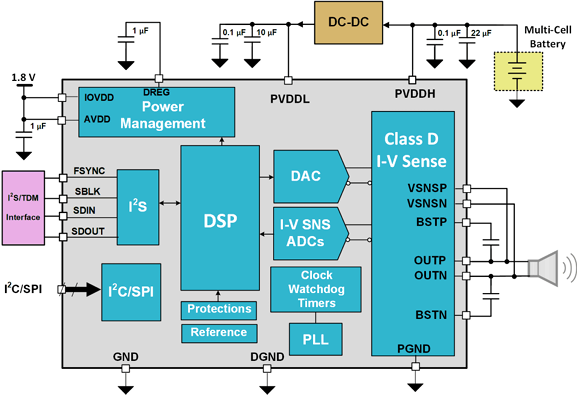
\includegraphics[width=\textwidth*3/4]{pictures/Blockschaltbild_TAS2781.png}
		\vspace{2mm}
		\caption{Blockschaltbild des TAS2781}
		\label{pic:blockschaltbild_TAS2781}
		\vspace{8mm}
	\end{subfigure}
	\begin{subfigure}{\textwidth}
		\centering
		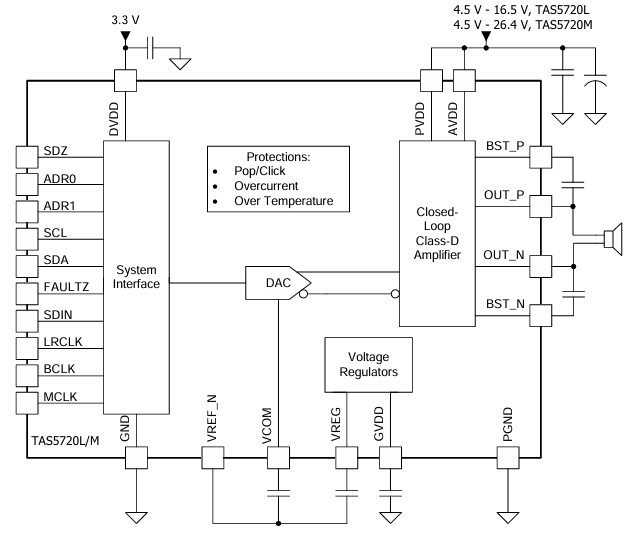
\includegraphics[width=\textwidth*3/4]{pictures/Blockschaltbild_TAS5720.png}
		\vspace{2mm}
		\caption{Blockschaltbild des TAS5720}
		\label{pic:blockschaltbild_TAS5720}
	\end{subfigure}
	\caption{Blockschaltbilder der potentiellen Endstufen}
\end{figure}
\subsubsection{Vergleich der Endstufen TAS2781 und TAS5720}Grundsätzlich wurde schnell klar, dass der \textbf{TAS2781} wesentlich komplexer und aufwändiger zu konfigurieren ist, aber einiges mehr an Features hat. Insbesondere die vier Speisungen, die teilweise auch vom Chip selber generiert werden können (Power Modes). Der \textbf{TAS5720} dagegen ist rudimentärer aufgebaut, hat aber einiges weniger an Features. Insbesondere der Limiter ist ein \textquotedbl harter\textquotedbl{} Limiter, begrenzt das Ausgangssignal pro Sample ohne einen zeitlichen Faktor. Somit wird das Signal lediglich begrenzt und es werden hörbare Verzerrungen erzeugt.
\begin{table}[H]
	\centering
	\setstretch{1.5}
	\begin{tabularx}{\textwidth*7/8}{>{\hsize=.65\hsize}XXX}
		&{\large \textbf{TAS2781}} & {\large \textbf{TAS5720}}\\\toprule
		\textbf{Output Power}&25W\newline{\small @ 1\% THD+N into 4 Ohm}&20W\newline{\small @ 0.15\% THD+N into 4 Ohm}\\\midrule
		\textbf{No. of Supplies}&4\newline {\small AVDD: 1.8 V\newline IOVDD: 1.8 V/ 3.3 V\newline PVDDL: 2.7 V to 5.5 V\newline PVDDH: 3 V to 24 V}&2\newline {\small Digital I/O: 3.3 V\newline 4.5 V to 16.5 V (TAS5720L)\newline 4.5 V to 26.4 V (TAS5720M)}\\\midrule
		\textbf{Input}&I2S/TDM\newline {\small 8 channels of 32 bits up to 192 KSPS}&TDM Audio Input\newline {\small Up to 8 Channels (32-bit, 48 kHz)}\\\midrule
		\textbf{Sample Rate}&16 kHz to 192 kHz&44.1 - 48 kHz {\small (Single Speed)}\newline 88.2 - 96 kHz {\small (Double Speed)}\\\midrule
		\textbf{Control Interface}&I2C with fast mode+ or SPI\newline Inter-chip communication bus&I2C Control With 8 Selectable I2C Address\\\midrule
		\textbf{No. of Configuration Registers}&156&9\\\midrule
		\textbf{Exposed Pad}&No&Yes\\\midrule
		\textbf{min. PSRR}&88 dB&50 dB\\\midrule
		\textbf{Special Features}&\textendash Low Voltage Signaling (LVS)\newline\textendash Noise Gate Mode\newline\textendash Supply Tracking Limiter\newline\textendash Brownout Prevention\newline\textendash ICC Pin and Inter-Chip Communication\newline\textendash Ultrasonic\newline\textendash Hard- \& Software Shutdown\newline\textendash Mute Mode\newline\textendash Beep Generator&Digital Clipper\newline\textendash Shutdown Mode (SDZ)\newline\textendash Sleep Mode\newline\textendash Mute Mode\\\midrule
		\textbf{Stückpreis auf DigiKey}&\$ 3.07&\$ 2.60\\\bottomrule
	\end{tabularx}
	\caption{Vergleich zwischen zwei Endstufen-ICs}
	\label{tab:Vergleich_TAS2781_TAS5720}
\end{table}\newpage
\noindent Ein weiterer wesentlicher Unterschied bestand in den Angaben zu THD+N\footnote{Total Harmonic Distrotion plus Noise} und zur Effizienz. Abbildung \ref{pic:thdn_vergleich} zeigt die THD+N Diagramme bei verschiedenen Speisespannungen. Zu beachten ist dass die y-Achse unterschiedlich skaliert sind: Beim TAS5720 sind diese in \% angegeben (Abbildung \ref{pic:thdn_perf_TAS5720}). Der tiefste Wert ist ungefähr bei 0.02\%, was $20\cdot log_{10}(\frac{0.02\%}{100}) = -73.98dB$ entspricht. Somit erzeugt der TAS2781 weniger (ca. 18dB tiefer) Verzerrungen und Rauschen.\\
Bei der Effizienz ist zu beachten, dass der TAS2781 verschiedene Power Modes hat, mit denen festgelegt werden kann wann und von welcher Speisung der Strom der internen Endstufe bezogen werden soll. Abbildung \ref{pic:TAS2781_powermodes} zeigt diese Operationsmodi. Der Vergleich zwischen Abbildungen \ref{pic:effizien_TAS2781_pwrmode0} und \ref{pic:effizien_TAS2781_pwrmode1} zeigt den Vorteil des Umschaltens: Die Effizienz bleibt auch bei niedrigen Signalpegeln über 30\% und zusammen\footnote{Zu beachten ist jedoch dass die X-Achse in Abbildung \ref{pic:effizien_TAS2781_pwrmode0} bei 0.0002W beginnt und in Abbildung \ref{pic:effizien_TAS2781_pwrmode1} bei 0.02W. Somit wird eine Effizienzsteigerung im Bereich von 10-20\% erreicht und nicht 30\%.}. Dies ist vor allem bei Batteriebetriebenen Anwendungen wichtig. Der Vergleich mit der Effizienz des TAS5720 zeigt, dass bei 5W Ausgangsleistung der TAS2781 \textit{ca.} 5-10\% effizienter arbeitet. Dies hängt allerdings bei beiden Modellen auch von der Speisespannung ab: Je höher desto weniger effizient.
\begin{figure}[H]
	\centering
	\begin{subfigure}{\textwidth}
		\centering
		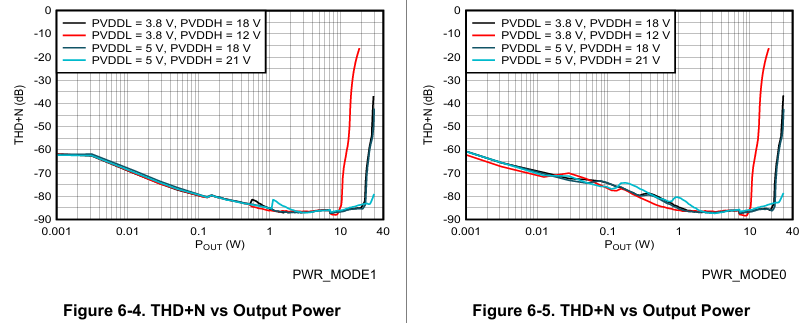
\includegraphics[width=\textwidth*7/8]{pictures/TAS2781_THDN_maxV.png}
		\vspace{2mm}
		\caption{THD+N Diagramm des TAS2781 (4 Ohm Last)}
		\label{pic:thdn_perf_TAS2781}
		\vspace{8mm}
	\end{subfigure}
	\begin{subfigure}{\textwidth}
		\centering
		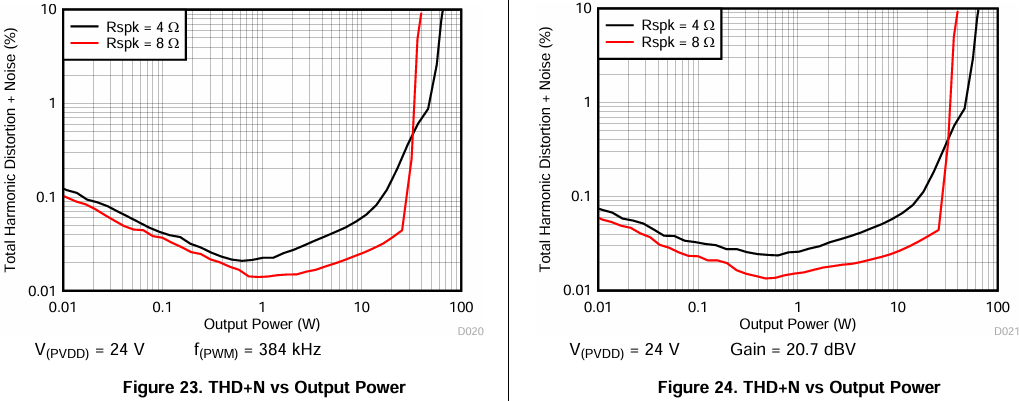
\includegraphics[width=\textwidth*7/8]{pictures/tas5720l_THDN_Vmax.png}
		\vspace{2mm}
		\caption{THD+N Diagramm des TAS5720}
		\label{pic:thdn_perf_TAS5720}
	\end{subfigure}
	\caption{THD+N Vergleich der Endstufen}
	\label{pic:thdn_vergleich}
\end{figure}
\begin{figure}[h]
	\centering
	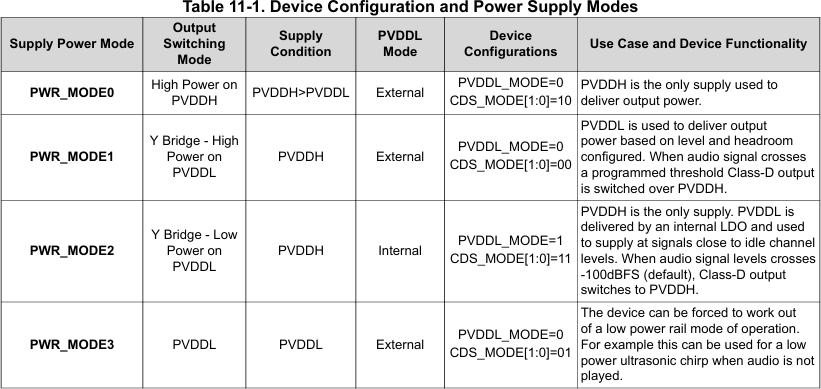
\includegraphics[width=\textwidth*7/8]{pictures/TAS2781_powermodes.png}
	\caption{Power Modes des TAS2781}
	\label{pic:TAS2781_powermodes}
\end{figure}
\begin{figure}[H]
	\centering
	\begin{subfigure}{\textwidth}
		\centering
		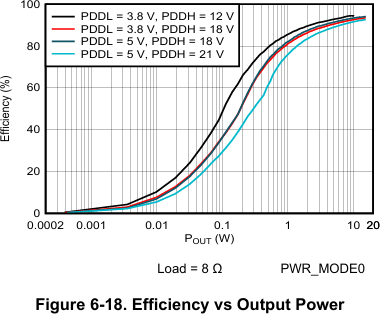
\includegraphics[width=\textwidth*4/8]{pictures/TAS2781_efficiency_powermode0.png}
		\vspace{2mm}
		\caption{Effizienz des TAS2781 (Power Mode 0)}
		\label{pic:effizien_TAS2781_pwrmode0}
		\vspace{8mm}
	\end{subfigure}
	\begin{subfigure}{\textwidth}
		\centering
		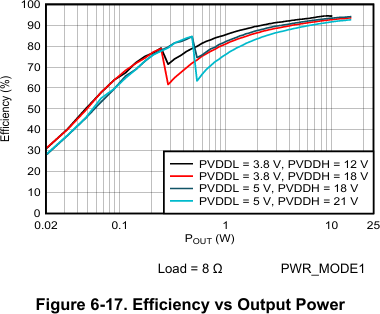
\includegraphics[width=\textwidth*4/8]{pictures/TAS2781_efficiency_powermode1.png}
		\vspace{2mm}
		\caption{Effizienz des TAS2781 (Power Mode 1)}
		\label{pic:effizien_TAS2781_pwrmode1}
	\end{subfigure}
\end{figure}
\begin{figure}[ht]\ContinuedFloat
	\centering
	\begin{subfigure}{\textwidth}
		\centering
		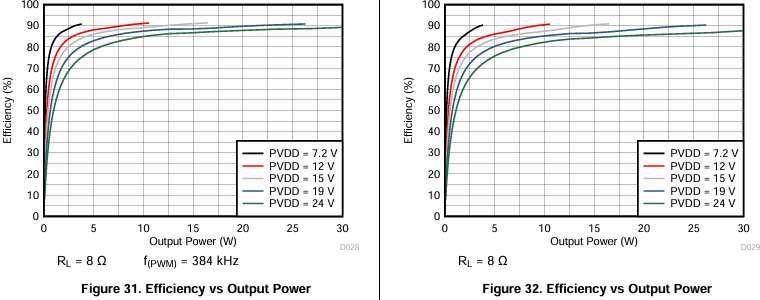
\includegraphics[width=\textwidth*7/8]{pictures/tas5720l_efficiency.png}
		\vspace{2mm}
		\caption{Effizienz des TAS5720}
		\label{pic:effizien_TAS5720}
	\end{subfigure}
	\caption{Vergleich der Effizienz der Endstufen}
	\label{pic:effizienz_vergleich}
\end{figure}
\subsubsection{Ausgangsstrom}
Aus der Effektivleistung und dem Crest-Faktor kann der Spitzenstrom berechnet werden:
\begin{equation}
	Iout_{ch(peak)} = \sqrt{\frac{P_{exciter(nom.)} \cdot Crest}{R_{exciter}}}  \rightarrow Iout_{ch(peak)} = \sqrt{\frac{5W \cdot 10^{\frac{6}{10}}}{4 Ohm}} = \textbf{2.23 A}
	\label{eq:peak_out_current_per_channel}
\end{equation}
Im Datenblatt des TAS5720 sind zwei Werte für den Maximalstrom angegeben: \textit{Peak output current} $I_{PK}$ und \textit{Overcurrent error (OCE)
threshold} $OCE_{(THRESH)}$. Während der erste Wert ein nominaler Grenzwert ist, zeigt der OCE-Wert die Stromstärke, bei der am Status-Pin \textit{FAULTZ} aktiviert wird (aktive low). Dieser Wert kann auch prozentual konfiguriert werden. Die Werte sind folgendermassen gegeben:
\begin{itemize}
	\item $I_{PK}$: \textbf{5 A}
	\item $OCE_{(THRESH)}$: \textbf{6 A}
\end{itemize}
Der Spitzenausgangsstrom ($I_{PK}$) des TAS5720 wird mit \textbf{5A} angegeben, somit kann die Endstufe auch die Spitzenströme gut liefern.\\
Im Datenblatt des TAS2781 sind lediglich das \textit{Output Over Current Limit on PVDDL} mit min. \textbf{2 A} und  \textit{Output Over Current Limit on PVDDH} mit min. \textbf{5.5 A} angegeben.
\begin{center}
	\begin{minipage}{\textwidth*7/8}
		\centering
		Somit können beide Endstufen die geforderten Spitzenströme liefern.
	\end{minipage}
\end{center}
\subsubsection{Fazit und Entscheid Endstufen}
Beide Endstufen bieten Leistungsmässig genug Headroom, um zu einem späteren Zeitpunkt auch 10W-Exciter zu treiben\footnote{Dies hätte Auswirkungen auf die Speisungsevaluation und soll dort entschieden werden.}. Die Unterschiede liegen hauptsächlich darin, dass der TAS2781 sehr viel mehr Funktionen und bessere Performance bietet, insbesondere im PSSR-Wert. Allerdings erfordernd die 156 Register einiges an Programmier- und Testaufwand. Zudem beinhaltet der TAS2781 einiges an Features, welche für dieses Projekt nicht relevant sind. Der Supply Tracking Limiter wäre sehr nützlich gewesen bei einer PoE-Speisung. Jedoch wird hier nun eine Netz-Betriebene Speisung verwendet und darum Spannungseinbrüche eher weniger zu erwarten bzw. werden vom externen Netzteil abgefangen.\\
\begin{center}
	\begin{minipage}{\textwidth*7/8}
		\centering
		{\large Daher wurde der \textbf{TAS5720} als kombinierter D/A-Wandler und Endstufe ausgewählt.\\
		Für eine optimierte Effizienz wurde zudem die Speisespannung auf \textbf{15V}, mit einer PWM-Frequenz von 384kHz festgelegt.}
	\end{minipage}
\end{center}